% version 1.00, date 07/03/16, auteur Mélissa Bignoux

\documentclass[asi]{picInsa}

%Pour le schéma d'architecture
\usepackage{etex}
\usepackage{tikz}
\usetikzlibrary{shapes,arrows,chains,backgrounds,fit}
%FIN Pour le shéma d'architecture

\DeclareGraphicsRule{*}{pdf}{*}{}
\usepackage{pdfpages}
\usepackage{vocabulaireUnipik}




\setcounter{secnumdepth}{4}
\setcounter{tocdepth}{4}
\newcommand{\ligneMaj}[3] {
	\rowcolor[gray]{0.55} \textbf{\textit{#1}} & #2  &  #3\\
	\hline
}
\newcommand{\ligneSup}[3] {
	\rowcolor[gray]{0.65} |\textunderscore \textbf{\textit{#1}} & #2  &  #3\\
	\hline
}
\newcommand{\ligneMed}[3] {
	\rowcolor[gray]{0.75} \hspace{0.25cm} |\textunderscore #1  & #2 & #3 \\
	\hline
}
\newcommand{\ligneSub}[3] {
	\rowcolor[gray]{0.85}  \hspace{0.5cm} |\textunderscore #1 & #2 & #3\\
	\hline
}
\newcommand{\ligneSubSub}[3] {
	\rowcolor[gray]{0.95}  \hspace{0.75cm} |\textunderscore #1 & #2 & #3\\
	\hline
}
\newcommand{\ligneTache}[3] {
	\hspace{1.00cm} |\textunderscore #1 & #2 & #3\\
	\hline
}
\title{\DCP{}}
\author{\Florian{}, \Kafui{}, \Melissa{}, \Julie{}, \Mathieu{}} %à changer


\titreGeneral{\DCP}
\sousTitreGeneral{\nomEquipe}
\titreAcronyme{\DCPCourt}

\titreDetaille{\DCPCourt\_D\_\nomEquipe\_l2}
\referenceVersion{\DCPCourt\_D\_\nomEquipe\_\versionPrive}
\auteurs{\Melissa{} \& \Florian{} \& \Michel{}}
\destinataires{\nomEquipe}
\resume{Le présent document contient la présentation du \DCP{} \nomEquipe.}
\motsCles{\DCPCourt{}}
\natureDerniereModification{Création}
\modeDiffusionControle{}

\begin{document}

\couverture{}

 \informationsGenerales{}
% version 1.00, date 29/02/16, auteur Michel Cressant
\begin{pagesService}
	\begin{historique}
		% nouvelles versions à rajouter AU-DESSUS en recopiant les lignes suivantes et en les modifiant :
		\unHistorique{1.00}{02/02/2016}{\Michel}{Création}{Toutes}

	\end{historique}

%        \begin{suiviDiffusions}
%
%            % On place ici les diffusions
%        	\unSuivi{1.00}{}{\nomEquipe{}}
%          
%          
%        \end{suiviDiffusions}

%%Signataires
        \begin{signatures}
	   \uneSignature{Vérificateur}{\RRS}{\Matthieu{}}{17/03/2016}{PGPic}
       \uneSignature{Validateur}{\CP{}}{\Sergi}{}{PGPic}
        \end{signatures}
	
	

	
	
\end{pagesService}


\tableofcontents

\setcounter{chapter}{0}


\chapter*{Introduction}
\label{intro}
% version 1.01 Date 24/03/2016	Auteur Mathieu Medici

\section*{Objet}
L'objectif de ce document est de présenter les principes et les procédures nécessaires à la mise en œuvre de la gestion des configurations prévue par la norme \isoNeufMilleUn.

\section*{Définition}

Le présent document établit les règles et la structure de la gestion des configurations qui doivent être suivies pendant toute la durée du \picCourt. Il contient :
\begin{itemize}
\item les règles de nommage;
\item la description des différents référentiels;
\item les règles spécifiques de \nomEquipe{};
\item la description de l'administration des configurations;
\item la description de la maîtrise des documents;
\item la description de la maîtrise des enregistrements;
\item les règles d'archivage.
\end{itemize}



\chapter{Cas d'utilisation}
\label{casUtilisation}
% version 1.00, date 20/02/16, auteur Michel Cressant
Ce chapitre décrit les différents cas d'utilisation pour chaque fonctionnalité.


\section{Fonctionnalité 8}
Ce paragraphe décrit les cas d'utilisation concernant la fonctionnalité 8 soit la géolocalisation. \\

La figure suivante (figure \ref{diagrammeCasUtilisation8}) indique les cas d'utilisation pour la géolocalisation.
\begin{figure}[H]
	\centering
	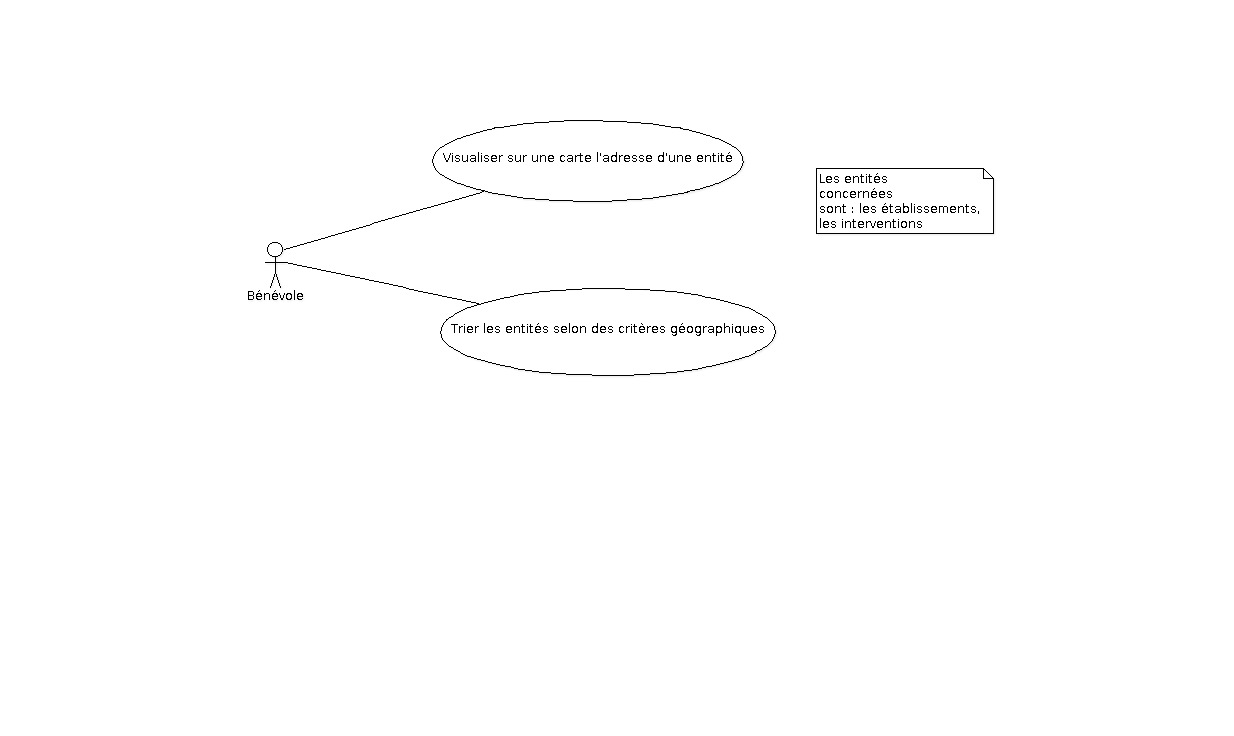
\includegraphics[scale=0.40]{casDUtilisation/images/fonctionnalite8Geolocalisation.png}
	\caption{Cas d'utilisation~: Géolocalisation }
	\label{diagrammeCasUtilisation8}
\end{figure}

\section{Fonctionnalité 9}
Ce paragraphe décrit les cas d'utilisation concernant la fonctionnalité 9 soit l'attribution de frimousse. \\

La figure suivante (figure \ref{diagrammeCasUtilisation9}) indique les cas d'utilisation pour l'attribution de frimousse.
\begin{figure}[H]
	\centering
	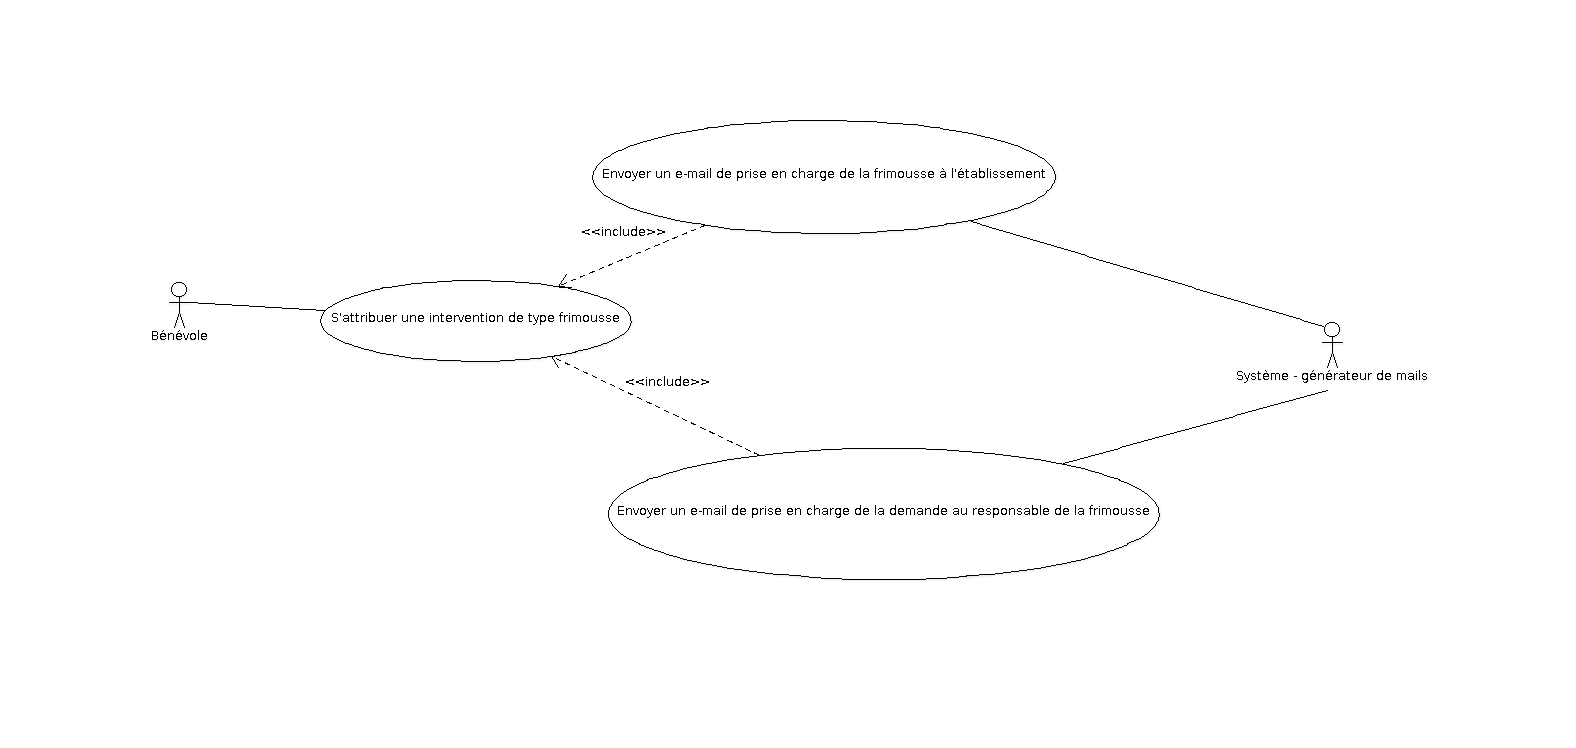
\includegraphics[scale=0.35]{casDUtilisation/images/fonctionnalite9Attribution.png}
	\caption{Cas d'utilisation~: Attribution de frimousse }
	\label{diagrammeCasUtilisation9}
\end{figure}

\section{Fonctionnalité 10}
Ce paragraphe décrit les cas d'utilisation concernant la fonctionnalité 10 soit la gestion des ventes. \\

La figure suivante (figure \ref{diagrammeCasUtilisation10}) indique les cas d'utilisation pour l'attribution de frimousse.
\begin{figure}[H]
	\centering
	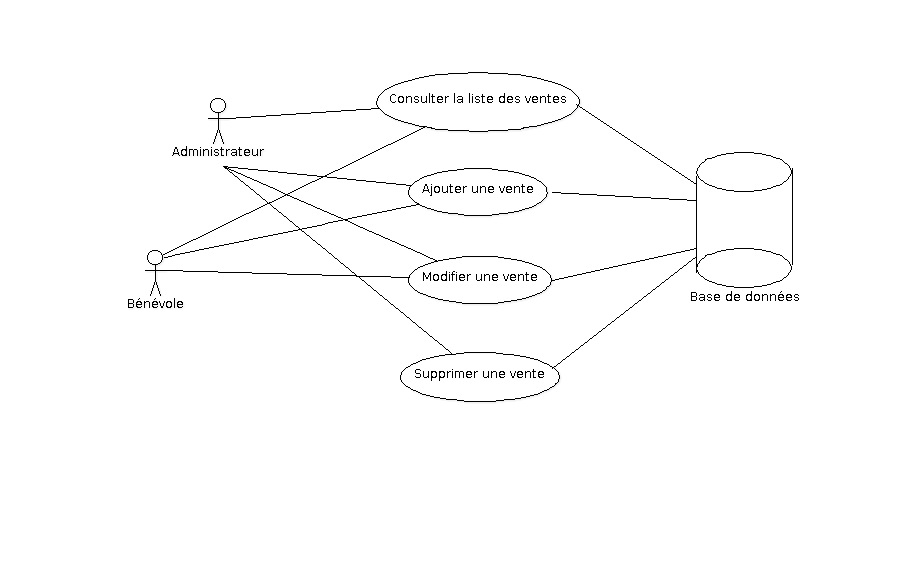
\includegraphics[scale=0.40]{casDUtilisation/images/fonctionnalite10Vente.png}
	\caption{Cas d'utilisation~: Gestion des ventes }
	\label{diagrammeCasUtilisation10}
\end{figure}


\chapter{Maquettes}
\label{maquettes}
% version 1.00, date 12/11/16, auteur Kafui Atanley
Ce chapitre présente les maquettes pour chaque fonctionnalité pour chaque fonctionnalité additionnelle du lot 3 par rapport au lot 2.


\section{Fonctionnalité 8}
Ce paragraphe décrit les maquettes concernant la fonctionnalité 8 soit la géolocalisation. \\

La figure suivante \ref{maquette8-1} montre la maquette d'une fiche descriptive d'une entité possédant une adresse. Un espace devra être réservé pour afficher la location de l'entité comme visible sur la fmaquette.
\begin{figure}[H]
	\centering
	\includegraphics[scale=0.40]{images/maquettes/fonctionnalite9Geolocalisation.png}
	\caption{Maquette~: Fiche descriptive d'une entité possédant une adresse}
	\label{maquette8-1}
\end{figure}
La figure suivante \ref{maquette8-2} présente la maquette des filtres de tri attendus sur la géolocalisation dans les pages permettant de lister les entités.
\begin{figure}[H]
	\centering
	\includegraphics[scale=0.40]{images/maquettes/fonctionnalite9Filtre.png}
	\caption{Maquette~: Modèle de filtre attendues dans les liste de tri}
	\label{maquette8-2}
\end{figure}

\section{Fonctionnalité 9}
Ce paragraphe décrit les maquettes concernant la fonctionnalité 9 soit l'attribution de frimousse. \\

La figure suivante montre l'email type de prise en charge d'une intervention de type frimousse.

La figure suivante montre la maquette de l'interface pour la prise en charge d'une intervention de type frimousse. L'utilisateur pourra s'attribuer une intervention de type frimousse via la liste d'intervention ou via la fiche descriptive de cette intervention.


\section{Fonctionnalité 10}
Ce paragraphe décrit les maquettes concernant la fonctionnalité 10 soit la gestion des ventes. \\

La figure suivante montre la maquette \ref{maquette10-5} de la page permettant d'ajouter une vente .
\begin{figure}[H]
	\centering
	\includegraphics[scale=0.40]{images/maquettes/fonctionnnalite10AjouterVente.png}
	\caption{Maquette~: Ajouter une vente}
	\label{maquette10-5}
\end{figure}

La figure suivante \ref{maquette10-3} montre la maquette de la page de la fiche descriptive d'une vente.
\begin{figure}[H]
	\centering
	\includegraphics[scale=0.40]{images/maquettes/fonctionnnalite10ConsulterVente.png}
	\caption{Maquette~: Consulter la fiche descriptive d'une vente}
	\label{maquette10-3}
\end{figure}

La figure suivante \ref{maquette10-4} Listing des ventes montre la maquette de la page permettant d'effectuer le listing des ventes.
\begin{figure}[H]
	\centering
	\includegraphics[scale=0.40]{images/maquettes/fonctionnalite10Ventes.png}
	\caption{Maquette~: Listing des ventes}
	\label{maquette10-4}
\end{figure}

La figure suivante \ref{maquette10-4} Listing des ventes montre la maquette de la page permettant d'effectuer le listing des ventes.

Il est possible de supprimer une vente à partir de la fiche descriptive d'une vente 




\begin{appendix}
\part*{Annexes}
\listoffigures
\addcontentsline{toc}{chapter}{Table des figures}
	 
\listoftables
\addcontentsline{toc}{chapter}{Liste des tableaux}
\end{appendix}
\pageQuatriemeCouverture

\end{document}